\chapter{Aplicație}
\section{Instrumente utilizate}
\Large{Am utilizat pentru dezvoltarea aplicației:}
\begin{itemize}
    \item {java 1.8}
    \item {JavaFX pentru interfață}
    \item {Intellij IDEA pentru scrierea si compilarea codului}
\end{itemize}
\section{Descriere}
Interfața grafică este alcătuită din:
\begin{itemize}
    \item butonul ← "Alegeți vectorul de sortat"
    \item TextArea ← unde se afiseaza vectorul nesortat si sortat
\end{itemize}
\newpage
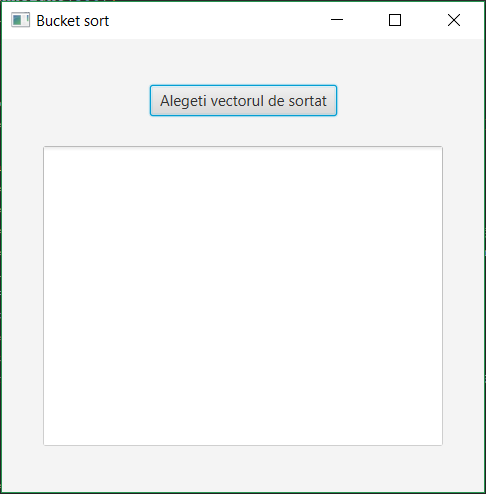
\includegraphics{aplicatie}\newline
După apăsarea butonului se deschide o fereastră de dialog care cere să se aleagă un fișier de tip text, care conține vectorul de sortat.\newline
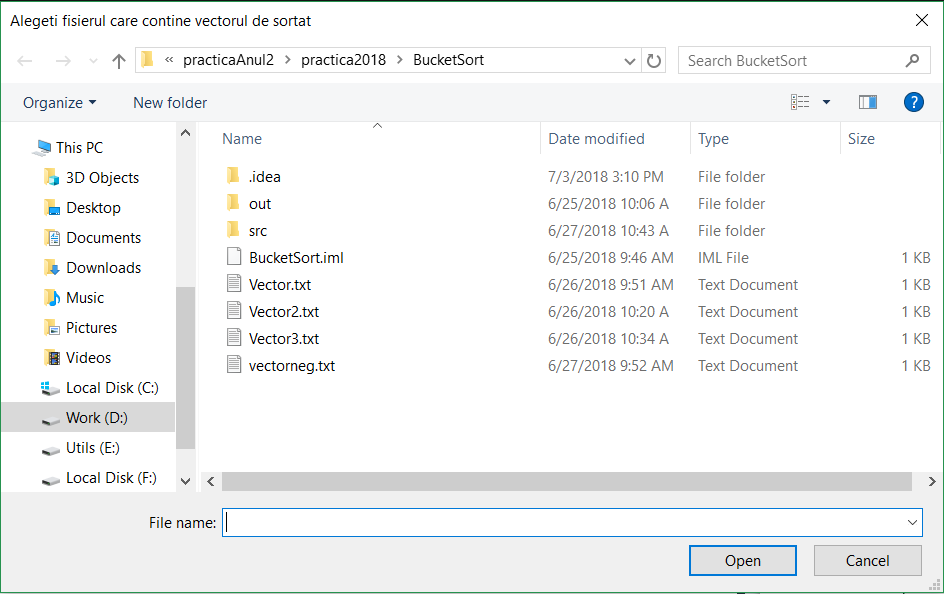
\includegraphics[scale=0.8]{fisier}\newline
După selectarea fișierului,care conține vectorul de sortat, se afișează în textarea vectorul din fișier si vectorul sortat.\newline
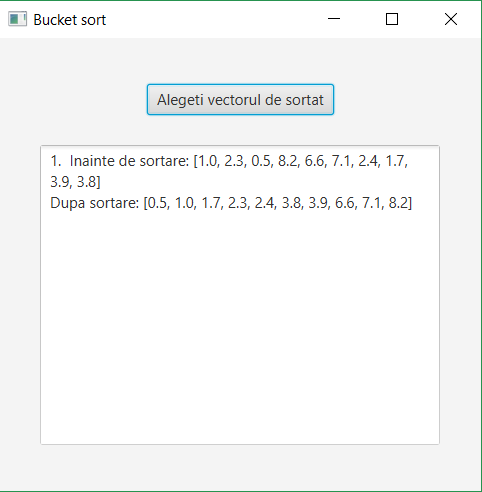
\includegraphics{sortat}
\section{Codul programului}
\subsection{Codul algoritmului}
\lstinputlisting[title=BucketSort.java ]{./BucketSort/src/BucketSort.java}
\subsection{Codul interfetei}
\lstinputlisting[title=Interfața.java ]{./BucketSort/src/Interfata.java}

